\documentclass[12pt]{article}

\usepackage{amsmath}
\usepackage{amssymb}
\usepackage{cmbright}
\usepackage{sfmath}
\usepackage{graphicx}
\usepackage[T1]{fontenc}
\usepackage{float}
\usepackage[margin=2.5cm]{geometry}
\usepackage{xcolor}
\usepackage{listings}
\usepackage{hyperref}

\usepackage[backend=biber,style=authoryear,
	maxcitenames=1,uniquelist=false,uniquename=false]{biblatex}
\addbibresource{references.bib}

% Code excerpts are pulled from code/gc_slip.py between '# begin:<name>' and
% '# end:<name>' comments, so the listings always match the code.
\lstset{
	language=Python,
	basicstyle=\ttfamily\footnotesize,
	columns=flexible,
	keepspaces=true,
	keywordstyle=\color{blue!60!black},
	commentstyle=\color{green!40!black},
	stringstyle=\color{red!50!black},
	showstringspaces=false,
	breaklines=true,
	frame=single,
	rulecolor=\color{black!25},
	numbers=left,
	numberstyle=\tiny\color{black!50},
	rangebeginprefix=\#\ begin:,
	rangeendprefix=\#\ end:,
	rangebeginsuffix=,
	rangeendsuffix=,
	includerangemarker=false,
}
\newcommand{\excerpt}[1]{\lstinputlisting[linerange=#1-#1]{code/gc_slip.py}}

\newcommand{\PV}{\mathrm{PV}\!\!}
\setlength{\emergencystretch}{2em}
\newcommand{\erfc}{\operatorname{erfc}}
\newcommand{\sgn}{\operatorname{sgn}}

\begin{document}

\title{Solving the slip equation with Gauss--Chebyshev quadrature}
\author{Kamal Ahmadov}
\date{\today}
\maketitle

This note derives a Gauss--Chebyshev collocation method for the fault-slip
problem of the note \texttt{2026-10-14\_slip} (its Eq.~2) and explains the
Python implementation in \texttt{code/gc\_slip.py}. The method follows
\textcite[Sec.~2 and 3.2]{ViescaGaragash2018}, who build on the quadratures of
\textcite{ErdoganGupta1972} and \textcite{ErdoganEtAl1973}.
Sections~\ref{sec:problem}--\ref{sec:discrete} contain the mathematics,
Section~\ref{sec:code} the code, and Section~\ref{sec:verification} the
verification. Section~\ref{sec:direct} describes a simpler direct scheme
(\texttt{explore/slip/gc.py}) for the case of a given pressure, and says when
each scheme is the right choice.

The folder contains
\begin{itemize}
	\item \texttt{code/gc\_slip.py}: the solver (listed in full in
	      Appendix~\ref{app:listing});
	\item \texttt{code/verify.py}: the checks quoted in
	      Section~\ref{sec:verification};
	\item \texttt{code/make\_figures.py}: writes the figures to
	      \texttt{figures/};
	\item \texttt{code/compare\_direct.py}: the comparison with the direct
	      scheme quoted in Section~\ref{sec:direct}.
\end{itemize}
The code needs only NumPy and SciPy (plus Matplotlib for the figures). Run
\texttt{verify.py} and \texttt{make\_figures.py} with
\texttt{code/} as the working directory or by their path. Rerun
\texttt{make\_figures.py} after changing the solver, so that the figures in
\texttt{figures/} stay in sync with the code.

%-------------------------------------------------------------------------------
\section{Problem statement}\label{sec:problem}

A fault $|x|<a$ slips under a pore-pressure perturbation
$p(x,t) = p_0 + \Delta p\, \hat p(x,t)$. On the slipping patch the shear stress
equals the Mohr--Coulomb strength,
\begin{equation}\label{eq:friction}
	\tau_0 + \Delta\tau(x,t) = f\,[\sigma_0 - p(x,t)], \qquad |x| < a,
\end{equation}
and the quasi-static change of shear stress due to slip $\delta$ is
\begin{equation}\label{eq:elastic}
	\Delta\tau(x,t) = \frac{G'}{\pi}\,\PV\int_{-a}^{a}
	\frac{\partial_s\delta(s,t)}{s-x}\,ds,
	\qquad G' = \frac{G}{2(1-\nu)},
\end{equation}
where $\PV$ denotes the Cauchy principal value. With
$\sigma_0' = \sigma_0 - p_0$, Eq.~\eqref{eq:friction} gives
$\Delta\tau = f\sigma_0' - \tau_0 - f\Delta p\,\hat p$. Scaling
\begin{equation*}
	\frac{x}{a} \to x, \qquad
	\frac{\delta\, G'}{f\Delta p\, a} \to \delta, \qquad
	\frac{\Delta\tau}{f\Delta p} \to \Delta\tau, \qquad
	\hat p \to p
\end{equation*}
and dropping hats, the problem becomes
\begin{equation}\label{eq:main}
	\boxed{\;T - p(a x) = \frac{1}{\pi}\,\PV\int_{-1}^{1}
		\frac{\delta'(s)}{s-x}\,ds, \qquad |x|<1,\;}
\end{equation}
with the stress-injection parameter \parencite{BhattacharyaViesca2019}
\begin{equation}\label{eq:T}
	T = \frac{f\sigma_0' - \tau_0}{f\Delta p}
	= \frac{1 - \tau_0/(f\sigma_0')}{\Delta p/\sigma_0'}.
\end{equation}
Eq.~\eqref{eq:main} is Eq.~2 of the slip note, since
$-\frac1\pi\int \delta'/(x-s)\,ds = \frac1\pi\int\delta'/(s-x)\,ds$. Two small
differences with that note:
\begin{itemize}
	\item the slip is scaled with $G'$ (not $G$); with $G$, a factor
	      $G'/G = 1/[2(1-\nu)]$ would multiply the integral;
	\item the shear stress in $T$ is the initial value $\tau_0$.
\end{itemize}

\paragraph{The pressure argument.} $p(\xi)$ is the scaled pressure as a function
of the \emph{physical} position $\xi$, in any convenient length unit. For
injection at constant pressure, $p(\xi) = \erfc|\xi|$ with
$\xi = x/\sqrt{4\alpha t}$ \parencite{BhattacharyaViesca2019}. The half-length
$a$ is then measured in units of $\sqrt{4\alpha t}$, and we call it
$\lambda = a/\sqrt{4\alpha t}$. In Eq.~\eqref{eq:main} the pressure is evaluated
at $\xi = a x$ because $x$ is in units of $a$. We write
\begin{equation*}
	\sigma(x) \equiv T - p(ax)
\end{equation*}
for the scaled load. It is the stress change that Eq.~\eqref{eq:main} requires
on the crack.

\paragraph{Conditions and unknowns.} The unknowns are the slip $\delta(x)$ on
$|x|<1$ and the half-length $a$. They are fixed by Eq.~\eqref{eq:main} together with
\begin{enumerate}
	\item zero slip at the tips, $\delta(\pm1)=0$;
	\item \emph{bounded stress at both tips}. A frictional crack without
	      fracture energy cannot carry a stress singularity, so the stress
	      intensity factors vanish, $K_\pm = 0$.
\end{enumerate}
Condition~(ii) is what determines $a$ (Section~\ref{sec:length}).

%-------------------------------------------------------------------------------
\section{Chebyshev toolbox}\label{sec:toolbox}

\subsection{Polynomials, roots and orthogonality}
With $x = \cos\theta$, the Chebyshev polynomials of the first and second kind are
\begin{equation*}
	T_k(x) = \cos k\theta, \qquad
	U_k(x) = \frac{\sin(k+1)\theta}{\sin\theta},
\end{equation*}
so $T_0 = U_0 = 1$, $T_1 = x$, $U_1 = 2x$, and $T_k' = k\,U_{k-1}$. We use the roots
\begin{align}
	s_j & = \cos\frac{j\pi}{n+1},       & j & = 1,\dots,n   &   & \text{(roots of } U_n),
	\label{eq:sj}                                                                         \\
	x_i & = \cos\frac{(i-\frac12)\pi}{n+1}, & i & = 1,\dots,n+1 &   & \text{(roots of } T_{n+1}),
	\label{eq:xi}
\end{align}
which interlace. Below we also write $\theta_j = \arccos s_j = j\pi/(n+1)$. The
polynomials are orthogonal with respect to their weights:
\begin{equation*}
	\int_{-1}^{1}\frac{T_kT_m}{\sqrt{1-x^2}}\,dx =
	\begin{cases} \pi & k=m=0 \\ \pi/2 & k=m>0 \\ 0 & k\neq m \end{cases},
	\qquad
	\int_{-1}^{1}\sqrt{1-x^2}\,U_kU_m\,dx = \frac{\pi}{2}\,\delta_{km}.
\end{equation*}

\subsection{Gauss--Chebyshev quadrature}
For the weight $\sqrt{1-s^2}$, the $n$-point Gauss rule is
\begin{equation}\label{eq:gauss}
	\int_{-1}^{1}\sqrt{1-s^2}\,g(s)\,ds \approx \sum_{j=1}^{n} w_j\, g(s_j),
	\qquad
	w_j = \frac{\pi}{n+1}\,(1-s_j^2) = \frac{\pi}{n+1}\sin^2\theta_j .
\end{equation}
It is exact when $g$ is a polynomial of degree $\le 2n-1$
\parencite{MasonHandscomb2003}. For the weight $1/\sqrt{1-x^2}$, the $(n+1)$-point
Gauss rule has nodes $x_i$ and equal weights $\pi/(n+1)$:
\begin{equation}\label{eq:gauss1}
	\int_{-1}^{1}\frac{g(x)}{\sqrt{1-x^2}}\,dx \approx \frac{\pi}{n+1}\sum_{i=1}^{n+1} g(x_i).
\end{equation}

\subsection{Finite Hilbert transforms}
Everything rests on Glauert's integral, for integer $m\ge0$ and $0<\theta<\pi$,
\begin{equation}\label{eq:glauert}
	\frac1\pi\,\PV\int_0^\pi \frac{\cos m\phi}{\cos\phi - \cos\theta}\,d\phi
	= \frac{\sin m\theta}{\sin\theta}.
\end{equation}
Substitute $s = \cos\phi$ and $x=\cos\theta$. Then
$\sqrt{1-s^2}\,U_k(s)\,ds = -\sin(k+1)\phi\,\sin\phi\,d\phi$, and
$\sin(k+1)\phi\sin\phi = \frac12[\cos k\phi - \cos(k+2)\phi]$. Applying
Eq.~\eqref{eq:glauert} to each cosine gives
$\frac12[\sin k\theta - \sin(k+2)\theta]/\sin\theta = -\cos(k+1)\theta$, that is,
\begin{equation}\label{eq:H2}
	\frac1\pi\,\PV\int_{-1}^{1}\frac{\sqrt{1-s^2}\,U_k(s)}{s-x}\,ds = -T_{k+1}(x),
	\qquad |x|<1,\; k\ge0 .
\end{equation}
This identity is the reason for the choice of basis. The Hilbert transform maps
$\sqrt{1-s^2}\,U_k$ to a single Chebyshev polynomial, and $T_0$ is never produced.

Off the crack, $|x|>1$, the integral is regular and equals
\begin{equation}\label{eq:H3}
	\frac1\pi\int_{-1}^{1}\frac{\sqrt{1-s^2}\,U_k(s)}{s-x}\,ds = -\rho(x)^{k+1},
	\qquad \rho(x) = x - \sgn(x)\sqrt{x^2-1},\quad |\rho|<1 .
\end{equation}
It follows by analytic continuation. The Cauchy integral
$\Psi(z) = \frac1\pi\int_{-1}^{1}\sqrt{1-s^2}\,U_k(s)/(z-s)\,ds$ is analytic off
$[-1,1]$ and vanishes at infinity. By the Plemelj formulae, its jump across the
cut (upper minus lower side) is $-2i\sqrt{1-x^2}\,U_k(x) = -2i\sin(k+1)\theta$.
Take the branch of $(z-\sqrt{z^2-1})^{k+1}$ that vanishes at infinity. It equals
$e^{\mp i(k+1)\theta}$ on the upper and lower sides of the cut, so it has the
same jump. By Liouville's theorem the two functions coincide. Off the cut,
$z-\sqrt{z^2-1} = \rho(x)$, which gives Eq.~\eqref{eq:H3}. On the cut, the
average of the two boundary values is $\cos(k+1)\theta = T_{k+1}(x)$, which
recovers Eq.~\eqref{eq:H2}. Since $\rho(\pm1) = \pm1$, the two expressions agree
at the tips.
Equation~\eqref{eq:H3} is checked to round-off in Section~\ref{sec:verification}.

%-------------------------------------------------------------------------------
\section{Structure of the solution}\label{sec:structure}

\subsection{Tip asymptotics fix the representation}
Near a tip with $K=0$, the stress is bounded and $\delta\sim(1-|x|)^{3/2}$, so
$\delta'\sim(1-|x|)^{1/2}$. For comparison, a crack with $K\ne0$ has
$\delta'\sim(1-|x|)^{-1/2}$. We therefore write
\begin{equation}\label{eq:ansatz}
	\delta'(s) = \sqrt{1-s^2}\;F(s),
	\qquad F(s) = \sum_{k=0}^{n-1} A_k\,U_k(s),
\end{equation}
with $F$ smooth up to the tips. The factor $\sqrt{1-s^2}$ is precisely the
weight of the $U_k$ \parencite[Table~1]{ViescaGaragash2018}. With this
representation, bounded stress at both tips is built in.

\subsection{Spectral form of the equation}
Inserting Eq.~\eqref{eq:ansatz} into Eq.~\eqref{eq:main} and using
Eq.~\eqref{eq:H2},
\begin{equation}\label{eq:spectral}
	\sigma(x) = T - p(ax) = -\sum_{k=0}^{n-1} A_k\, T_{k+1}(x).
\end{equation}
Expand the load as $\sigma(x) = \sum_{m\ge0} c_m T_m(x)$, with
$c_m = \frac{2-\delta_{m0}}{\pi}\int_{-1}^{1}\sigma T_m/\sqrt{1-x^2}\,dx$.
Matching coefficients gives
\begin{equation}\label{eq:match}
	c_0 = 0, \qquad A_k = -c_{k+1}\quad (k\ge0).
\end{equation}
The first relation is a \emph{solvability condition} on the load. The second
relation solves for the slip once the load is known.

\subsection{Crack half-length: the \texorpdfstring{$K=0$}{K=0} condition}\label{sec:length}
Written out, $c_0=0$ reads
\begin{equation}\label{eq:length}
	\boxed{\;T = \frac1\pi\int_{-1}^{1}\frac{p(as)}{\sqrt{1-s^2}}\,ds\;}
\end{equation}
In words, the Chebyshev-weighted average of the pressure over the crack equals
$T$. This is the classical condition for a non-singular crack tip,
$\int_{-a}^{a}\Delta\tau/\sqrt{a^2-x^2}\,dx = 0$
\parencite{Rice1968}; see also Eq.~11 of \textcite{ViescaGaragash2018}. It
contains only $a$, so the half-length can be found \emph{before} the slip.

To see the link with the stress intensity factors, recall that
\parencite{Rice1968}
\begin{equation*}
	K_\pm \propto \int_{-1}^{1}\sigma(s)\sqrt{\frac{1\pm s}{1\mp s}}\,ds .
\end{equation*}
The sum and the difference of the two weights are
$2/\sqrt{1-s^2}$ and $2s/\sqrt{1-s^2}$. So $K_+=K_-=0$ is equivalent to
$c_0 = c_1 = 0$. The representation \eqref{eq:ansatz} has bounded stress built
in, and $c_1$ appears through the closure of the crack:
\begin{equation}\label{eq:closure}
	\delta(1)-\delta(-1) = \int_{-1}^{1}\sqrt{1-s^2}\,F(s)\,ds = \frac\pi2 A_0 = -\frac\pi2\,c_1 .
\end{equation}
For a pressure profile symmetric about the injection point, $\sigma$ is even, so
$c_1 = 0$ and $\delta(\pm1)=0$ holds automatically. For an asymmetric profile,
$c_1=0$ is a second condition. It determines a second unknown, the position of
the crack centre. The code treats only the symmetric case.

\subsection{Example: injection at constant pressure}\label{sec:erfc}
For $p(\xi)=\erfc|\xi|$, Eq.~\eqref{eq:length} becomes
\begin{equation}\label{eq:lambda}
	T = \frac1\pi\int_{-1}^{1}\frac{\erfc(\lambda|s|)}{\sqrt{1-s^2}}\,ds .
\end{equation}
The half-length grows as $a = \lambda\sqrt{4\alpha t}$ with $\lambda(T)$
constant, so the solution is self-similar. Two limits follow directly from
Eq.~\eqref{eq:lambda}:
\begin{itemize}
	\item $\lambda\gg1$ (critically stressed fault, $T\ll1$). The pressure is
	      concentrated where $1/\sqrt{1-s^2}\approx1$, so
	      $T\approx\frac2\pi\int_0^\infty\erfc(\lambda s)\,ds
		      = 2/(\pi^{3/2}\lambda)$ and
	      \begin{equation*}
		      \lambda \approx \frac{2}{\pi^{3/2}\,T}.
	      \end{equation*}
	\item $\lambda\ll1$ (marginally pressurized fault, $1-T\ll1$). Using
	      $\erfc(\lambda|s|)\approx1-2\lambda|s|/\sqrt\pi$ and
	      $\int_0^1 s/\sqrt{1-s^2}\,ds=1$ gives $T\approx1-4\lambda/\pi^{3/2}$ and
	      \begin{equation*}
		      \lambda \approx \frac{\pi^{3/2}}{4}\,(1-T).
	      \end{equation*}
\end{itemize}
For small $T$, the slipping patch extends far beyond the pressurized zone
($\lambda>1$).

%-------------------------------------------------------------------------------
\section{Discretisation}\label{sec:discrete}

\subsection{Unknowns}
The unknowns are the nodal values $F_j = F(s_j)$, $j=1,\dots,n$, at the roots of
$U_n$, Eq.~\eqref{eq:sj}. Through $n$ values, $F$ is represented by its
interpolating polynomial of degree $n-1$. This is the truncated series in
Eq.~\eqref{eq:ansatz}.

\subsection{Quadrature of the singular integral}\label{sec:singquad}
Following \textcite{ErdoganEtAl1973}, we apply the Gauss rule \eqref{eq:gauss} to
the singular integral as if it were regular:
\begin{equation}\label{eq:singquad}
	\frac1\pi\,\PV\int_{-1}^{1}\frac{\sqrt{1-s^2}\,F(s)}{x-s}\,ds
	\approx \frac1\pi\sum_{j=1}^{n}\frac{w_j\,F(s_j)}{x-s_j}.
\end{equation}
This is not exact for general $x$. However, it \textbf{is exact at the
collocation points $x=x_i$ (the roots of $T_{n+1}$) whenever $F$ is a polynomial
of degree $\le 2n$}. The proof has two steps.

\emph{Lemma.} For $|x|<1$, $x\neq s_j$,
\begin{equation}\label{eq:lemma}
	\sum_{j=1}^{n}\frac{w_j}{x-s_j}
	= \PV\int_{-1}^{1}\frac{\sqrt{1-s^2}}{x-s}\,ds - \pi\,\frac{T_{n+1}(x)}{U_n(x)}
	= \pi x - \pi\,\frac{T_{n+1}(x)}{U_n(x)} .
\end{equation}
To prove it, note that $[U_n(x)-U_n(s)]/(x-s)$ is a polynomial of degree $n-1$
in $s$, so Eq.~\eqref{eq:gauss} integrates it exactly. Because $U_n(s_j)=0$, the
quadrature sum is $U_n(x)\sum_j w_j/(x-s_j)$. Evaluating the two integrals with
Eq.~\eqref{eq:H2} ($k=n$ and $k=0$) gives Eq.~\eqref{eq:lemma}. At $x=x_i$ we
have $T_{n+1}(x_i)=0$ and $U_n(x_i)\ne0$ (the roots interlace), so the rule is
exact for $F\equiv1$.

\emph{General $F$.} Split
$F(s)/(x-s) = [F(s)-F(x)]/(x-s) + F(x)/(x-s)$. The first term is a polynomial
in $s$ of degree $\deg F - 1 \le 2n-1$, which the Gauss rule integrates exactly.
The second term is exact at $x_i$ by the lemma. \hfill$\square$

\subsection{Collocation system}
Equation~\eqref{eq:main} reads
$\frac1\pi\PV\int\delta'(s)/(x-s)\,ds = p(ax)-T$. Collocating it at the $n+1$
points $x_i$ with Eq.~\eqref{eq:singquad} gives
\begin{equation}\label{eq:system}
	\sum_{j=1}^{n} H_{ij}\,F_j = p(a x_i) - T, \quad i=1,\dots,n+1,
	\qquad
	H_{ij} = \frac{w_j}{\pi\,(x_i-s_j)} = \frac{1-s_j^2}{(n+1)(x_i-s_j)} .
\end{equation}
This is $n+1$ equations for $n$ unknowns $F_j$ plus the unknown $a$, as in
Eq.~10 of \textcite{ViescaGaragash2018}.

\subsection{Discrete solvability is the discrete \texorpdfstring{$K=0$}{K=0} condition}
The columns of $H$ sum to zero. Since $T_{n+1}(s) = 2^n\prod_i(s-x_i)$,
\begin{equation*}
	\sum_{i=1}^{n+1}\frac{1}{x_i-s_j} = -\frac{T_{n+1}'(s_j)}{T_{n+1}(s_j)}
	= -\frac{(n+1)\,U_n(s_j)}{T_{n+1}(s_j)} = 0 .
\end{equation*}
Summing Eq.~\eqref{eq:system} over $i$ therefore eliminates every $F_j$ and leaves
\begin{equation}\label{eq:dlength}
	\boxed{\;T = \frac{1}{n+1}\sum_{i=1}^{n+1} p(a x_i)\;}
\end{equation}
This is Eq.~\eqref{eq:length} evaluated with the Gauss rule \eqref{eq:gauss1}. So
the overdetermined system is consistent exactly when the discrete $K=0$
condition holds, and this condition determines $a$ independently of $F$.

Given Eq.~\eqref{eq:dlength}, the solution $F$ is unique. By exactness,
$(HF)_i = \sum_k A_k T_{k+1}(x_i)$. The polynomials $T_1,\dots,T_n$ evaluated at
$n+1$ distinct points are linearly independent, so $H$ has full column rank $n$.

\subsection{Recovering the slip}
The coefficients $A_k$ follow from the nodal values through the discrete
orthogonality relation
\begin{equation*}
	\sum_{j=1}^{n}\sin(k+1)\theta_j\,\sin(m+1)\theta_j = \frac{n+1}{2}\,\delta_{km},
	\qquad 0\le k,m\le n-1,
\end{equation*}
which gives
\begin{equation}\label{eq:B}
	A_k = \sum_{j=1}^{n} B_{kj}F_j, \qquad
	B_{kj} = \frac{2}{n+1}\,\sin\theta_j\,\sin(k+1)\theta_j .
\end{equation}
Integrating Eq.~\eqref{eq:ansatz} from the tip $x=-1$, where $\delta=0$, gives
$\delta(x) = \sum_k A_k I_k(x)$ with
\begin{equation*}
	I_k(x) = \int_{-1}^{x}\sqrt{1-s^2}\,U_k(s)\,ds
	= \frac12\int_\theta^\pi[\cos k\phi - \cos(k+2)\phi]\,d\phi,
\end{equation*}
which evaluates to
\begin{equation*}
	I_k(x) = \begin{cases}
		\frac12\left(\pi-\theta+\frac12\sin2\theta\right), & k=0,\\[3pt]
		\frac12\left(\dfrac{\sin(k+2)\theta}{k+2} - \dfrac{\sin k\theta}{k}\right), & k\ge1,
	\end{cases}
\end{equation*}
where $\theta=\arccos x$. In matrix form,
\begin{equation}\label{eq:S}
	\delta(x_q) = \sum_{j=1}^{n} S_{qj}F_j, \qquad S = I\,B,
\end{equation}
which is the integration matrix of \textcite[Sec.~2.4, Tables~2 and
4]{ViescaGaragash2018}. It integrates the interpolant of $F$ exactly, so the
evaluation points $x_q$ are arbitrary. At the far tip, $I_k(1) = \frac\pi2\delta_{k0}$,
which recovers Eq.~\eqref{eq:closure}.

\subsection{Stress on and off the crack}\label{sec:stress}
By Eqs.~\eqref{eq:H2} and~\eqref{eq:H3}, the stress change produced by the
solution is
\begin{equation}\label{eq:stress}
	\Delta\tau(x) = \frac1\pi\int_{-1}^{1}\frac{\delta'(s)}{s-x}\,ds =
	\begin{cases}
		-\sum_k A_k\,T_{k+1}(x),     & |x|\le1, \\
		-\sum_k A_k\,\rho(x)^{k+1}, & |x|>1 .
	\end{cases}
\end{equation}
On the crack, this equals $T-p(ax_i)$ at the collocation points and interpolates
between them. Off the crack, it is needed to check that the solution is
admissible. The fault outside the slipping patch must not exceed its strength,
$\tau_0+f\Delta p\,\Delta\tau \le f(\sigma_0 - p)$, or in scaled form
\begin{equation}\label{eq:admissible}
	\Delta\tau(x) \le T - p(ax), \qquad |x|>1 .
\end{equation}

\subsection{Algorithm}
\begin{enumerate}
	\item Choose $n$ and compute $s_j$, $w_j$ and $x_i$ (Eqs.~\ref{eq:sj}, \ref{eq:xi}
	      and~\ref{eq:gauss}).
	\item Solve the scalar equation \eqref{eq:dlength} for $a$.
	\item Solve the consistent $(n+1)\times n$ system \eqref{eq:system} for $F_j$.
	\item Compute the slip from Eq.~\eqref{eq:S} and, if needed, the stress from
	      Eq.~\eqref{eq:stress}.
\end{enumerate}

%-------------------------------------------------------------------------------
\section{The code}\label{sec:code}

The listings below are excerpts of \texttt{code/gc\_slip.py}. The line numbers
are those of the file.

\paragraph{Nodes and weights} (Eqs.~\ref{eq:sj}, \ref{eq:xi} and~\ref{eq:gauss}).
\excerpt{nodes}

\paragraph{Singular-integral matrix} $H_{ij}$ of Eq.~\eqref{eq:system}. It uses
NumPy broadcasting: \texttt{x[:, None] - s[None, :]} is the $(n+1)\times n$
matrix $x_i - s_j$. No entry is singular because the two point sets interlace.
\excerpt{hilbert}

\paragraph{Half-length} from the discrete $K=0$ condition \eqref{eq:dlength}.
\texttt{brentq} needs the residual $g(a) = \frac1{n+1}\sum_i p(ax_i) - T$ to
change sign over \texttt{bracket}. For a pressure that decreases with $|\xi|$
from $p(0)=1$ to $0$, $g$ decreases from $1-T$ towards $-T$. For even $n$,
however, $x=0$ is a collocation point, so $g(\infty) = 1/(n+1) - T$. A
\texttt{ValueError} from \texttt{brentq} therefore means that either $T$ lies
outside $(0,1)$ or $n$ is too small to resolve the pressurized zone
(Section~\ref{sec:resolution}).
\excerpt{crack_length}

\paragraph{Chebyshev coefficients} $B_{kj}$ of Eq.~\eqref{eq:B}. The array
\texttt{k} is a column and \texttt{th} a row, so the result is the $n\times n$
matrix $B_{kj}$.
\excerpt{coefficients}

\paragraph{Integration matrix} $S = IB$ of Eq.~\eqref{eq:S}. \texttt{Phi} holds
$I_k(x_q)$: its first column is the $k=0$ case and the other columns are
$k=1,\dots,n-1$. The \texttt{clip} protects \texttt{arccos} from round-off just
outside $[-1,1]$.
\excerpt{integration}

\paragraph{Stress change} on and off the crack, Eq.~\eqref{eq:stress}, from the
coefficients $A_k$. Inside, $T_{k+1}(x) = \cos[(k+1)\arccos x]$. Outside,
$\rho^{k+1}$ decays geometrically because $|\rho|<1$.
\excerpt{stress}

\paragraph{Driver.} \texttt{solve\_slip} performs steps 1--3 of the algorithm.
It returns a \texttt{SlipSolution}, whose methods \texttt{slip} and
\texttt{stress} perform step 4 at any points. Equation~\eqref{eq:system} is
consistent, so \texttt{lstsq} returns its exact solution. The stored
\texttt{residual} is a self-check and is at round-off level ($\sim10^{-14}$)
in every case we ran. Dropping any one row of $H$ and calling
\texttt{np.linalg.solve} would give the same $F$.
\excerpt{solve}

\paragraph{Units.} \texttt{sol.a} is in the length unit of the argument of
\texttt{p}. \texttt{sol.slip(x)} takes $x$ in units of $a$ and returns
$\delta\,G'/(f\Delta p\,a)$. \texttt{sol.stress(x)} returns $\Delta\tau/(f\Delta p)$.

\paragraph{Usage.} Injection at constant pressure with $T=0.5$:
\begin{lstlisting}[numbers=none]
import numpy as np
from scipy.special import erfc
from gc_slip import solve_slip

sol = solve_slip(lambda xi: erfc(np.abs(xi)), T=0.5, n=256)
sol.a                                # lambda = a / sqrt(4 alpha t): 0.79162
sol.slip(np.linspace(-1, 1, 201))    # delta G' / (f Dp a) on x/a in [-1, 1]
\end{lstlisting}
For a pressure profile from a run file (\texttt{fracinj.io.read\_hdf5}), first
sort the positions with \texttt{io.sort\_fields}. Then interpolate the scaled
pressure at one time index, for example
\texttt{p = lambda xi: np.interp(xi, x\_grid, (p\_grid - p0)/dp)}, with
\texttt{x\_grid} measured from the injection point. Two cautions apply.
\texttt{np.interp} holds the end value beyond the grid, so check that $a$ is
smaller than the fracture half-length. The piecewise-linear interpolant also
has kinks, so expect algebraic rather than spectral convergence
(Section~\ref{sec:convergence}).

%-------------------------------------------------------------------------------
\section{Verification}\label{sec:verification}

All numbers below are printed by \texttt{code/verify.py}.

\subsection{Identities}
\begin{enumerate}
	\item \emph{Exactness of the singular quadrature.} We take $n=16$ and
	      $F=U_m$, and compare $HF$ with the exact value $T_{m+1}(x_i)$. The
	      error is below $2\times10^{-14}$ for $m = 0, 1, 15, 16, 32 = 2n$, and
	      $O(1)$ for $m = 33 = 2n+1$. This confirms the degree-$2n$ exactness proved
	      above.
	\item \emph{Column sums.} $\max_j|\sum_i H_{ij}| = 5\times10^{-15}$.
	\item \emph{Off-crack transform} \eqref{eq:H3}. It matches adaptive
	      quadrature to $10^{-16}$ at $x=1.3$ and $x=-2$, for $k=0,\dots,5$.
\end{enumerate}

\subsection{Manufactured solution}
Take $\delta = (1-x^2)^{3/2}$, which has bounded stress at both tips. Then
$\delta' = -3x\sqrt{1-x^2}$, so $F = -3x = -\frac32U_1$, and
Eq.~\eqref{eq:spectral} gives $\Delta\tau = \frac32T_2 = 3x^2-\frac32$. This is
Eq.~\eqref{eq:main} with $T=0$ and $p(\xi) = \frac32 - 3\xi^2$. For this pressure,
Eq.~\eqref{eq:dlength} gives $\frac32 - \frac32a^2 = 0$, because the mean of
$x_i^2$ is $\frac12$. Hence $a=1$, as it must be. Off the crack,
Eq.~\eqref{eq:stress} gives $\Delta\tau = \frac32\rho^2$. For $n = 2$, $4$ and
$32$, the solver reproduces $a$, $\delta$, and $\Delta\tau$ (on and off the
crack) to $4\times10^{-14}$ or better.

\subsection{Injection at constant pressure}
Figure~\ref{fig:lambda} compares $\lambda(T)$ from Eq.~\eqref{eq:dlength} with
adaptive quadrature of Eq.~\eqref{eq:lambda} and with the two limits of
Section~\ref{sec:erfc}. Table~\ref{tab:lambda} lists the relative errors.
Figure~\ref{fig:slip} shows the slip profiles and the stress change. On the
crack, $\Delta\tau$ coincides with $T-p$. At the tips it is continuous and
bounded, which is the $K=0$ condition. Off the crack it stays below $T-p$, so
the admissibility condition~\eqref{eq:admissible} holds.

\begin{table}[H]
	\centering
	\caption{Half-length $\lambda$ for $p=\erfc|\xi|$ (adaptive quadrature of
		Eq.~\eqref{eq:lambda}), its two limits, and the relative error of
		Eq.~\eqref{eq:dlength} for three values of $n$. A dash means that
		Eq.~\eqref{eq:dlength} has no root because the pressurized zone is not
		resolved (Section~\ref{sec:resolution}).}
	\label{tab:lambda}
	\begin{tabular}{ccccccc}
		\hline
		$T$  & $\lambda$ & $\frac{2}{\pi^{3/2}T}$ & $\frac{\pi^{3/2}}{4}(1-T)$ & $n=32$             & $n=128$            & $n=512$            \\
		\hline
		0.02 & 17.968    & 17.959                 & 1.3642                     & --                 & $3.4\times10^{-2}$ & $2.0\times10^{-3}$ \\
		0.1  & 3.6405    & 3.5917                 & 1.2529                     & $2.0\times10^{-2}$ & $1.3\times10^{-3}$ & $7.9\times10^{-5}$ \\
		0.5  & 0.7916    & 0.7183                 & 0.6960                     & $1.1\times10^{-3}$ & $7.4\times10^{-5}$ & $4.7\times10^{-6}$ \\
		0.9  & 0.1398    & 0.3991                 & 0.1392                     & $7.7\times10^{-4}$ & $5.0\times10^{-5}$ & $3.2\times10^{-6}$ \\
		0.99 & 0.0139    & 0.3628                 & 0.0139                     & $7.6\times10^{-4}$ & $4.9\times10^{-5}$ & $3.1\times10^{-6}$ \\
		\hline
	\end{tabular}
\end{table}

\begin{figure}[H]
	\centering
	\begin{minipage}{0.49\linewidth}
		\centering
		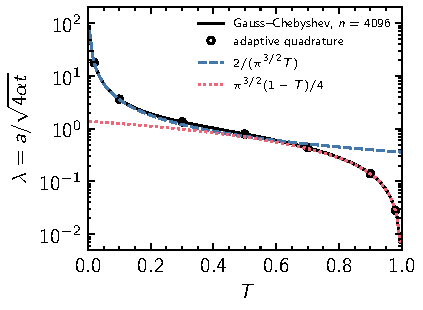
\includegraphics[width=\linewidth]{figures/crack-length.pdf}
	\end{minipage}\hfill
	\begin{minipage}{0.49\linewidth}
		\centering
		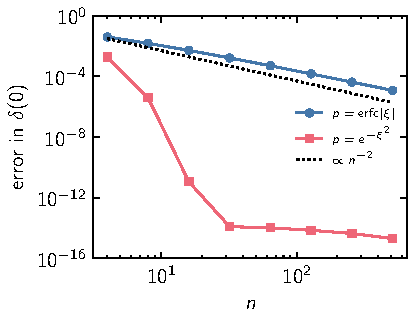
\includegraphics[width=\linewidth]{figures/convergence.pdf}
	\end{minipage}
	\caption{Left: half-length $\lambda = a/\sqrt{4\alpha t}$ for injection at
		constant pressure. The curve is Eq.~\eqref{eq:dlength} with $n=4096$, the
		circles are adaptive quadrature of Eq.~\eqref{eq:lambda}, and the dashed
		and dotted lines are the critically stressed and marginally pressurized
		limits. Right: error in $\delta(0)$ at $T=0.5$ against $n$ (reference
		$n=4001$) for the kinked profile $\erfc|\xi|$ and the analytic profile
		$e^{-\xi^2}$.}
	\label{fig:lambda}
\end{figure}

\begin{figure}[H]
	\centering
	\begin{minipage}{0.49\linewidth}
		\centering
		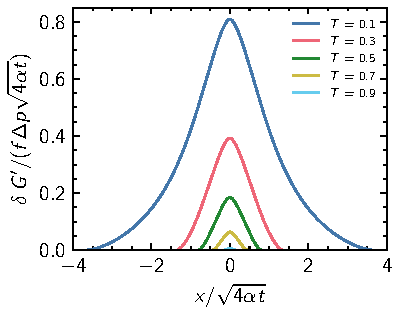
\includegraphics[width=\linewidth]{figures/slip-profiles.pdf}
	\end{minipage}\hfill
	\begin{minipage}{0.49\linewidth}
		\centering
		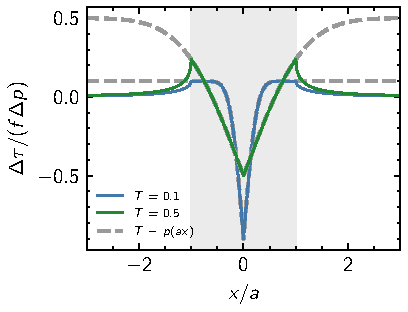
\includegraphics[width=\linewidth]{figures/stress.pdf}
	\end{minipage}
	\caption{Injection at constant pressure, $n=512$. Left: slip in diffusion
		units, $\lambda\,\delta(x/a)$ against $x/\sqrt{4\alpha t} = \lambda x$.
		Right: stress change $\Delta\tau$ from Eq.~\eqref{eq:stress} (solid) and
		the scaled strength excess $T-p(ax) = [f(\sigma_0-p)-\tau_0]/(f\Delta p)$
		(dashed) against $x/a$. The shaded band is
		the slipping patch.}
	\label{fig:slip}
\end{figure}

\subsection{Convergence}\label{sec:convergence}
The right panel of Figure~\ref{fig:lambda} shows two behaviours.
\begin{itemize}
	\item For the analytic profile $p=e^{-\xi^2}$, convergence is
	      \emph{spectral}: the error reaches round-off by $n\approx32$. For this
	      profile Eq.~\eqref{eq:length} has the closed form
	      $T = e^{-\lambda^2/2}I_0(\lambda^2/2)$. At $T=0.5$, where
	      $\lambda = 1.3242673802$, Eq.~\eqref{eq:dlength} gives $\lambda$ to a
	      relative error of $3\times10^{-9}$ with $n=8$ and to round-off with
	      $n=16$.
	\item For $p=\erfc|\xi|$, convergence is algebraic, close to $n^{-2}$. The
	      cause is the kink of $\erfc|\xi|$ at $\xi=0$. A discontinuity in
	      $d\sigma/dx$ at an interior point produces a logarithmic singularity in
	      $\delta''$ there \parencite[App.~A]{ViescaGaragash2018}, which a
	      polynomial $F$ cannot represent well.
\end{itemize}
Any pressure interpolated piecewise-linearly from a grid behaves like the second
case.

\subsection{Resolution requirement}\label{sec:resolution}
The nodes cluster at the tips. Near the centre their spacing is about $\pi/n$ in
units of $a$, while the pressure varies over a length $1/\lambda$ in the same
units. Resolving the pressurized zone therefore requires
\begin{equation*}
	n \gg \pi\lambda \approx \frac{2}{\sqrt\pi\,T} \quad (T\ll1).
\end{equation*}
At $T=0.02$ ($\lambda\approx18$), $n=32$ cannot even bracket the root of
Eq.~\eqref{eq:dlength}, while $n=512$ gives $\lambda$ to 0.2\%
(Table~\ref{tab:lambda}). The cost is a dense $(n+1)\times n$ least-squares
problem, so $n$ of a few thousand is still cheap. The direct scheme of
Section~\ref{sec:direct} has the same resolution requirement but costs only
$O(n^2)$.

%-------------------------------------------------------------------------------
\section{A direct scheme for a given pressure}\label{sec:direct}

When the pressure is given, the linear solve of Section~\ref{sec:discrete} can
be skipped. The collocation system \eqref{eq:system} has an explicit inverse,
and \texttt{explore/slip/gc.py} implements it.\footnote{\raggedright\texttt{gc} is also the
	name of a built-in Python module, so \texttt{import gc} never loads this file.
	\texttt{code/compare\_direct.py} loads it by path.} The numbers below are
printed by \texttt{code/compare\_direct.py}.

\paragraph{Inversion formula.} Glauert's integral \eqref{eq:glauert}, with
$s=\cos\phi$, also gives the companion of Eq.~\eqref{eq:H2}:
\begin{equation}\label{eq:H1}
	\frac1\pi\,\PV\int_{-1}^{1}\frac{T_m(s)}{\sqrt{1-s^2}\,(s-x)}\,ds =
	\begin{cases} U_{m-1}(x), & m\ge1,\\ 0, & m=0. \end{cases}
\end{equation}
Apply it to $\sigma = \sum_m c_mT_m$ and use $A_k = -c_{k+1}$ from
Eq.~\eqref{eq:match}. This gives
\begin{equation}\label{eq:inverse}
	F(x) = \sum_k A_k U_k(x)
	= \frac1\pi\,\PV\int_{-1}^{1}\frac{\sigma(s)}{\sqrt{1-s^2}\,(x-s)}\,ds
	= -\frac1\pi\,\PV\int_{-1}^{1}\frac{p(as)}{\sqrt{1-s^2}\,(x-s)}\,ds .
\end{equation}
This is the classical solution of Eq.~\eqref{eq:main} that is bounded at both
ends \parencite{Muskhelishvili1953}. The constant $T$ drops out (the $m=0$ case
of Eq.~\ref{eq:H1}), so $T$ enters only through $a$.

\paragraph{Discretisation.} Sample the pressure at the $n+1$ points $x_i$,
Eq.~\eqref{eq:xi}, and evaluate Eq.~\eqref{eq:inverse} with the first-kind Gauss
rule \eqref{eq:gauss1}:
\begin{equation}\label{eq:direct}
	F_j = -\frac{1}{n+1}\sum_{i=1}^{n+1}\frac{p(ax_i)}{s_j-x_i},
	\qquad j=1,\dots,n .
\end{equation}
The half-length is again the root of Eq.~\eqref{eq:dlength}. Repeat the argument
of Section~\ref{sec:singquad} with $T_{n+1}$ and $U_n$ exchanged. It shows that this rule is exact
at the $s_j$ for polynomial densities of degree $\le 2n+2$. In particular, it is
exact for the degree-$n$ interpolant $P$ of $p(a\,\cdot)$ through the $x_i$.

The collocation solution is also exact for this load. To see this, note that
$-\sum_kA_kT_{k+1}$ and $T-P$ are both polynomials of degree $n$, and they agree
at the $n+1$ points $x_i$. Both schemes therefore return the exact $F$ for the
load $T-P$, and their $F_j$ are identical: Eq.~\eqref{eq:direct} is the
explicit inverse of $H$.

\paragraph{Slip.} In $\theta$, the points $x_i$ (at $(i-\frac12)\pi/(n+1)$) lie
midway between the $\theta_j = j\pi/(n+1)$. Integrating from the tip $x=-1$
($\theta=\pi$) with the composite midpoint rule in $\theta$ gives
\begin{equation}\label{eq:midpoint}
	\delta(x_i) = \int_{\arccos x_i}^{\pi}\sin^2\phi\;F(\cos\phi)\,d\phi
	\approx \sum_{j=i}^{n} w_jF_j ,
\end{equation}
a reversed cumulative sum. The half-interval next to the tip, where the integrand
is $O(n^{-2})$, is dropped. The rule is second-order accurate in $n$.

\paragraph{Stress off the crack.} For $|x|>1$, the first line of
Eq.~\eqref{eq:stress} is a regular integral. The Gauss rule \eqref{eq:gauss}
gives $\Delta\tau(x) \approx -\frac1\pi\sum_jw_jF_j/(x-s_j)$. It loses accuracy
only within a few node spacings of the tips.

\paragraph{Correspondence with \texttt{gc.py}.} The code counts nodes differently
and swaps two names:
\begin{itemize}
	\item its \texttt{n} is the number of pressure nodes ($n+1$ here);
	\item \texttt{s} holds our $x_i$ and \texttt{x} our $s_j$;
	\item \texttt{phi} is $F$.
\end{itemize}

\paragraph{Comparison.} Write $N=n+1$ for the number of pressure nodes. The
checks are:
\begin{itemize}
	\item \emph{Slip gradient.} On the same nodes, the two schemes give the same
	      $a$. The $F_j$ agree to $2\times10^{-11}$ or better for $p = \erfc|\xi|$,
	      $e^{-\xi^2}$ and a uniform patch, with $N\le257$.
	\item \emph{Slip.} Table~\ref{tab:direct} lists the maximum slip error at the
	      $x_i$. For the patch, the reference is the exact solution, with
	      $a = l/\sin(\pi T/2)$ from Eq.~\eqref{eq:length}. For the other two
	      profiles, the reference is the collocation scheme with $n=8000$. There,
	      the two schemes differ by $4\times10^{-8}$.
	\item \emph{Run time.} For $p=\erfc|\xi|$, the direct scheme takes 0.006~s
	      at $N=1024$ and 0.12~s at $N=4096$. The collocation scheme takes 0.29~s
	      and 7.7~s.
\end{itemize}

\begin{table}[H]
	\centering
	\caption{Maximum slip error at the nodes $x_i$, $T=0.5$ (patch: $T=0.6$,
		half-width $l=5$ in units of the pressure argument).}
	\label{tab:direct}
	\begin{tabular}{lcccc}
		\hline
		& \multicolumn{2}{c}{$N=64$} & \multicolumn{2}{c}{$N=1024$} \\
		pressure        & direct             & collocation         & direct             & collocation         \\
		\hline
		uniform patch   & $5.6\times10^{-3}$ & $4.4\times10^{-3}$  & $6.6\times10^{-4}$ & $5.9\times10^{-4}$  \\
		$\erfc|\xi|$    & $5.3\times10^{-5}$ & $2.3\times10^{-4}$  & $2.1\times10^{-7}$ & $1.6\times10^{-6}$  \\
		$e^{-\xi^2}$    & $1.2\times10^{-4}$ & $1.0\times10^{-14}$ & $4.8\times10^{-7}$ & $1.7\times10^{-14}$ \\
		\hline
	\end{tabular}
\end{table}

The patch converges slowly in both schemes, for two reasons. The pressure jump
makes $F$ singular at $x=\pm l/a$. In addition, the residual of
Eq.~\eqref{eq:dlength} is a staircase in $a$, so $a$ is found only to within
a node spacing.

\paragraph{Which scheme to use.} Use the direct scheme whenever the load on
the crack is known in advance, as for a given pressure with $K=0$ at the tips.
It needs no linear solve and costs $O(n^2)$. For kinked or discontinuous
pressures (erfc, a patch, or pressure interpolated from simulation data), its
midpoint-rule slip is as accurate as the spectral integration of
Section~\ref{sec:discrete}, or more accurate. Only for an analytic pressure does the
collocation slip win.

Keep the collocation scheme (\texttt{code/gc\_slip.py}) for problems in which the
stress on the crack depends on the slip, because then no closed-form inverse
exists. Examples are slip-weakening or rate-dependent friction, cohesive zones,
coupling with dilatancy or permeability, and a toughness criterion $K=K_c$. The
matrix $H$, or the Jacobian of a Newton iteration built from it, is then the
general tool.

%-------------------------------------------------------------------------------
\section{Remarks and extensions}

\begin{itemize}
	\item \emph{Time dependence.} With a constant friction coefficient, the
	      quasi-static problem has no memory. The solution at time $t$ follows
	      from $p(\cdot,t)$ alone, provided that slip does not decrease anywhere
	      (no unloading). For injection at constant pressure, the solution is
	      self-similar, $a=\lambda\sqrt{4\alpha t}$, and slip grows monotonically.
	\item \emph{Asymmetric pressure.} Replace $p(ax)$ by $p(b+ax)$ and treat the
	      crack centre $b$ as a second unknown. The two conditions are
	      Eq.~\eqref{eq:dlength} and the discrete closure $A_0 = 0$ (see
	      Eq.~\ref{eq:closure}). By the discrete orthogonality of $T_1$ and
	      $T_{k+1}$ on the nodes $x_i$, the closure is equivalent to
	      $\sum_i x_i\,p(b+ax_i) = 0$, so both conditions again involve only the
	      pressure.
	\item \emph{Fracture energy.} If the tips must satisfy $K=K_c\neq0$, use the
	      first-kind representation $\delta' = F/\sqrt{1-s^2}$
	      \parencite[Sec.~3.1]{ViescaGaragash2018}. It has nodes
	      $s_j = \cos[(j-\frac12)\pi/n]$, $j=1,\dots,n$, and collocation points
	      $x_i=\cos(i\pi/n)$, $i=1,\dots,n-1$, together with the closure
	      $\sum_jF_j=0$. Then $K_\pm\propto F(\pm1)$, which follows from the
	      $F_j$ by the end-point interpolation vectors of their Table~3. Setting
	      $F(1)$ to the value that corresponds to $K_c$ fixes $a$.
\end{itemize}

\printbibliography

\appendix
\section{Full listing of \texttt{code/gc\_slip.py}}\label{app:listing}
\lstinputlisting{code/gc_slip.py}

\end{document}
